\documentclass[border={40.500000bp 20.000000bp 20.000000bp 20.000000bp}, 12pt]{standalone}
\pdfinfoomitdate=1
\pdftrailerid{}
\pdfsuppressptexinfo=1
\pdfinfo{ /Creator () /Producer () }

\usepackage{tikz}
\usepackage{xcolor}
\usetikzlibrary{shapes.misc}
\usetikzlibrary{backgrounds}

\definecolor{dotColorA}{HTML}{000000}
\definecolor{dotColorB}{HTML}{000000}
\definecolor{dotColorC}{HTML}{000000}
\definecolor{dotColorD}{HTML}{000000}
\definecolor{dotColorE}{HTML}{000000}
\definecolor{dotColorF}{HTML}{000000}
\definecolor{dotColorG}{HTML}{000000}

\definecolor{labelBgColorA}{HTML}{000000}
\definecolor{labelBgColorB}{HTML}{000000}
\definecolor{labelBgColorC}{HTML}{000000}
\definecolor{labelBgColorD}{HTML}{000000}
\definecolor{labelBgColorE}{HTML}{000000}
\definecolor{labelBgColorF}{HTML}{000000}
\definecolor{labelBgColorG}{HTML}{000000}

\definecolor{labelTextColorA}{HTML}{FFFFFF}
\definecolor{labelTextColorB}{HTML}{FFFFFF}
\definecolor{labelTextColorC}{HTML}{FFFFFF}
\definecolor{labelTextColorD}{HTML}{FFFFFF}
\definecolor{labelTextColorE}{HTML}{FFFFFF}
\definecolor{labelTextColorF}{HTML}{FFFFFF}
\definecolor{labelTextColorG}{HTML}{FFFFFF}

\definecolor{linkColorA}{HTML}{000000}
\definecolor{linkColorB}{HTML}{000000}
\definecolor{linkColorC}{HTML}{000000}
\definecolor{linkColorD}{HTML}{000000}
\definecolor{linkColorE}{HTML}{000000}
\definecolor{linkColorF}{HTML}{000000}
\definecolor{linkColorG}{HTML}{000000}

\def\textA{1977 - A New Hope}
\def\textB{1980 - The Empire Strikes Back}
\def\textC{1984 - Return of the Jedi}
\def\textD{1999 - The Phantom Menace}
\def\textE{2002 - Attack of the Clones}
\def\textF{2005 - Revenge of the Sith}
\def\textG{2015 - The Force Awakens}

\begin{document}
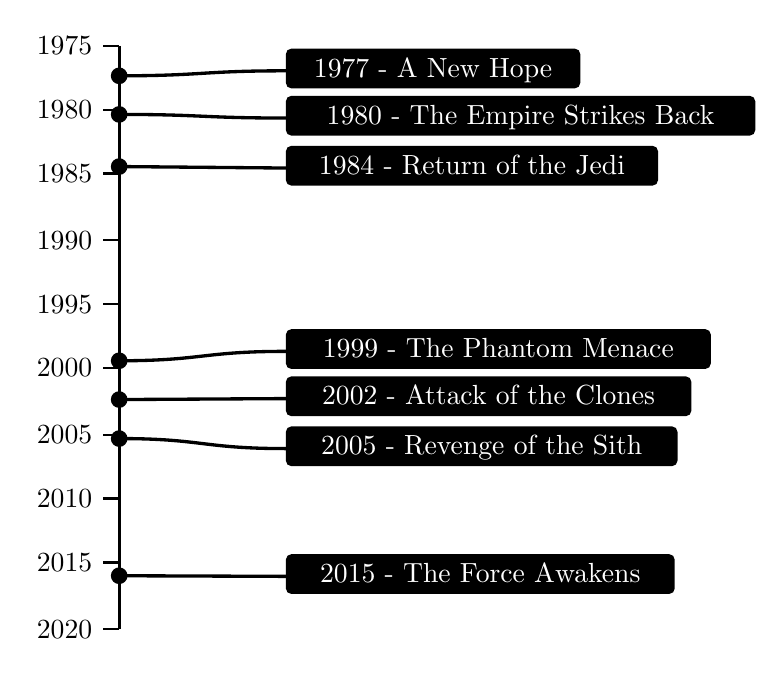
\begin{tikzpicture}[x=1bp,y=-1bp]

% shift for the margin
\begin{scope}[shift={(40, 20)}]
% main layer
\begin{scope}[shift={(0, 0)}]
% axis
\begin{scope}
\draw[very thick] (0, 0) -- (0, 210);
\end{scope}

% axis layer
\begin{scope}
\begin{scope}[shift={(0, 0)}]
\draw[thick] (0, 0) -- (-6pt, 0)
node[anchor=east] {1975};
\end{scope}
\begin{scope}[shift={(0, 23)}]
\draw[thick] (0, 0) -- (-6pt, 0)
node[anchor=east] {1980};
\end{scope}
\begin{scope}[shift={(0, 46)}]
\draw[thick] (0, 0) -- (-6pt, 0)
node[anchor=east] {1985};
\end{scope}
\begin{scope}[shift={(0, 70)}]
\draw[thick] (0, 0) -- (-6pt, 0)
node[anchor=east] {1990};
\end{scope}
\begin{scope}[shift={(0, 93)}]
\draw[thick] (0, 0) -- (-6pt, 0)
node[anchor=east] {1995};
\end{scope}
\begin{scope}[shift={(0, 116)}]
\draw[thick] (0, 0) -- (-6pt, 0)
node[anchor=east] {2000};
\end{scope}
\begin{scope}[shift={(0, 140)}]
\draw[thick] (0, 0) -- (-6pt, 0)
node[anchor=east] {2005};
\end{scope}
\begin{scope}[shift={(0, 163)}]
\draw[thick] (0, 0) -- (-6pt, 0)
node[anchor=east] {2010};
\end{scope}
\begin{scope}[shift={(0, 186)}]
\draw[thick] (0, 0) -- (-6pt, 0)
node[anchor=east] {2015};
\end{scope}
\begin{scope}[shift={(0, 210)}]
\draw[thick] (0, 0) -- (-6pt, 0)
node[anchor=east] {2020};
\end{scope}
\end{scope}

% link layer
\begin{scope}
\draw[color=linkColorA, very thick] (0.00000000, 10.79589012) .. controls
(30.00000000, 10.79589012) and (30.00000000, 9.00000000) .. (60.00000000, 9.00000000);
\draw[color=linkColorB, very thick] (0.00000000, 24.69708262) .. controls
(30.00000000, 24.69708262) and (30.00000000, 26.00000000) .. (60.00000000, 26.00000000);
\draw[color=linkColorC, very thick] (0.00000000, 43.46624787) .. controls
(30.00000000, 43.46624787) and (30.00000000, 44.00000000) .. (60.00000000, 44.00000000);
\draw[color=linkColorD, very thick] (0.00000000, 113.38106899) .. controls
(30.00000000, 113.38106899) and (30.00000000, 110.00000000) .. (60.00000000, 110.00000000);
\draw[color=linkColorE, very thick] (0.00000000, 127.34614566) .. controls
(30.00000000, 127.34614566) and (30.00000000, 127.00000000) .. (60.00000000, 127.00000000);
\draw[color=linkColorF, very thick] (0.00000000, 141.38788330) .. controls
(30.00000000, 141.38788330) and (30.00000000, 145.00000000) .. (60.00000000, 145.00000000);
\draw[color=linkColorG, very thick] (0.00000000, 190.77086882) .. controls
(30.00000000, 190.77086882) and (30.00000000, 191.00000000) .. (60.00000000, 191.00000000);
\end{scope}

% label layer
\begin{scope}
\begin{scope}[shift={(60, 1)}]
\fill[color=labelBgColorA, rounded corners=2pt]
(0, 0) rectangle (106, 14.33331) node[midway, yshift=-.75bp, anchor=center, text=labelTextColorA] {\strut \textA};
\end{scope}
\begin{scope}[shift={(60, 18)}]
\fill[color=labelBgColorB, rounded corners=2pt]
(0, 0) rectangle (169, 14.33331) node[midway, yshift=-.75bp, anchor=center, text=labelTextColorB] {\strut \textB};
\end{scope}
\begin{scope}[shift={(60, 36)}]
\fill[color=labelBgColorC, rounded corners=2pt]
(0, 0) rectangle (134, 14.33331) node[midway, yshift=-.75bp, anchor=center, text=labelTextColorC] {\strut \textC};
\end{scope}
\begin{scope}[shift={(60, 102)}]
\fill[color=labelBgColorD, rounded corners=2pt]
(0, 0) rectangle (153, 14.33331) node[midway, yshift=-.75bp, anchor=center, text=labelTextColorD] {\strut \textD};
\end{scope}
\begin{scope}[shift={(60, 119)}]
\fill[color=labelBgColorE, rounded corners=2pt]
(0, 0) rectangle (146, 14.33331) node[midway, yshift=-.75bp, anchor=center, text=labelTextColorE] {\strut \textE};
\end{scope}
\begin{scope}[shift={(60, 137)}]
\fill[color=labelBgColorF, rounded corners=2pt]
(0, 0) rectangle (141, 14.33331) node[midway, yshift=-.75bp, anchor=center, text=labelTextColorF] {\strut \textF};
\end{scope}
\begin{scope}[shift={(60, 183)}]
\fill[color=labelBgColorG, rounded corners=2pt]
(0, 0) rectangle (140, 14.33331) node[midway, yshift=-.75bp, anchor=center, text=labelTextColorG] {\strut \textG};
\end{scope}
\end{scope}

% dots
\begin{scope}
\draw node [circle, inner sep=0pt, minimum size=6bp, 
fill=dotColorA] at (0, 10.795890) {};
\draw node [circle, inner sep=0pt, minimum size=6bp, 
fill=dotColorB] at (0, 24.697083) {};
\draw node [circle, inner sep=0pt, minimum size=6bp, 
fill=dotColorC] at (0, 43.466248) {};
\draw node [circle, inner sep=0pt, minimum size=6bp, 
fill=dotColorD] at (0, 113.381069) {};
\draw node [circle, inner sep=0pt, minimum size=6bp, 
fill=dotColorE] at (0, 127.346146) {};
\draw node [circle, inner sep=0pt, minimum size=6bp, 
fill=dotColorF] at (0, 141.387883) {};
\draw node [circle, inner sep=0pt, minimum size=6bp, 
fill=dotColorG] at (0, 190.770869) {};
\end{scope}

\end{scope}
\end{scope}
\end{tikzpicture}
\end{document}